% ============================================================
%  Blowup Algebras  --  polished version
%  The preamble below is self-contained so the file compiles on its own.
%  Merge the macro block with your existing preamble and delete duplicates.
% ============================================================
\documentclass[11pt]{article}
\usepackage[margin=1in]{geometry}
\usepackage{fullpage}
\usepackage{mdframed}
\usepackage{multicol}
\usepackage{colonequals}
\usepackage{algpseudocode}
\usepackage{algorithm}
\usepackage[most, breakable]{tcolorbox}
\usepackage[all]{xy}
\usepackage{proof}
\usepackage{mathtools}
\usepackage{bbm}
\usepackage{amssymb}
\usepackage{amsthm}
\usepackage{amsmath}
\usepackage{amsxtra}
\usepackage{tikz-cd}
\usepackage{enumitem}
\usepackage{euler}
\usepackage{mathpazo}
\usepackage{wrapfig}

\newtheorem{theorem}{Theorem}[section]
\newtheorem{theorem*}{Theorem}
\newtheorem{definition}[theorem]{Definition}
\newtheorem{corollary}{Corollary}[theorem]
\newtheorem{lemma}[theorem]{Lemma}
\newtheorem{lemmact}[theorem]{Lemmact}
\newtheorem{proposition}[theorem]{Proposition}
\newtheorem{remark}[theorem]{Remark}
\newtheorem{example}{Example}[section]


% \newtheorem*{exercisehelper}{Exercise.}
% \newenvironment{exercise}[1]{%
%   \IfBlankTF{#1}
%     {\renewcommand{\exercisehelper}{\textbf{Exercise} \unskip}}
%     {\renewcommand\exercisehelper{\textbf{Exercise #1}}}%
%   \exercisehelper
% }{\endexercisehelper}

\theoremstyle{remark}
\newtheorem{exercise}{Exercise}[section]
\newtheorem*{solution}{Solution}
\newtheorem*{notation}{Notation}
\newcommand{\mathcat}[1]{\textup{\textbf{\textsf{#1}}}} % for defined terms

\newenvironment{problem}[1]
{ \begin{tcolorbox}[breakable]\noindent\textbf{Problem #1}.}
{\vskip 6pt \end{tcolorbox}}

\newenvironment{enumalph}
{\begin{enumerate}\renewcommand{\labelenumi}{\textnormal{(\alph{enumi})}}}
{\end{enumerate}}

\newenvironment{enumroman}
{\begin{enumerate}\renewcommand{\labelenumi}{\textnormal{(\roman{enumi})}}}
{\end{enumerate}}

\newcommand{\defi}[1]{\textsf{#1}} % for defined terms



\setlength{\hfuzz}{4pt}

\let\H\relax
\let\P\relax
\newcommand{\bb}{\mathbb}
\newcommand{\A}{\mathbb A}
\newcommand{\H}{\mathbb H}
\newcommand{\E}{\mathbb E}
\newcommand{\P}{\mathbb P}
\newcommand{\C}{\mathbb C}
\newcommand{\I}{\mathbb I}
\newcommand{\K}{\mathbb K}
\newcommand{\N}{\mathbb N}
\newcommand{\Q}{\mathbb Q}
\newcommand{\R}{\mathbb R}
\newcommand{\Z}{\mathbb Z}
\newcommand{\F}{\mathbb F}
\newcommand{\V}{\mathbb V}
\newcommand{\br}{\mathbf{r}}
\newcommand{\RP}{\mathbb{RP}}
\newcommand{\CP}{\mathbb{CP}}
\newcommand{\nbit}[1]{\{0, 1\}^{#1}}
\newcommand{\bits}{\{0, 1\}^{n}}
\newcommand{\bbni}{\bigbreak \noindent}
\newcommand{\norm}[1]{\left\vert\left\vert#1\right\vert\right\vert}
\newcommand{\dbar}{\overline{\partial}}
\let\d\relax
\newcommand{\d}{\partial}
\newcommand{\e}{\epsilon}
\newcommand{\cO}{\mathcal{O}}
\newcommand{\FF}{\mathcal{F}}
\newcommand{\cG}{\mathcal{G}}
\newcommand{\HH}{\mathcal{H}}
\newcommand{\EE}{\mathcal{E}}
\newcommand{\CC}{\mathcal{C}}
\newcommand{\DD}{\mathcal{D}}
\newcommand{\PP}{\mathcal{P}}
\newcommand{\iso}{\cong}
\newcommand{\tism}{Talked to Sair Shaikh'26}
\DeclareMathOperator{\fm}{\mathfrak{m}}
\DeclareMathOperator{\fn}{\mathfrak{n}}
\DeclareMathOperator{\fp}{\mathfrak{p}}
\DeclareMathOperator{\fq}{\mathfrak{q}}
\DeclareMathOperator{\fM}{\mathfrak{M}}
\DeclareMathOperator{\fP}{\mathfrak{P}}


\newcommand{\Frac}{\text{Frac}}
\newcommand{\Tor}{\text{Tor}}
\newcommand{\Ext}{\text{Ext}}
\newcommand{\gr}{\text{gr}}
\newcommand{\pd}{\text{pd}}
\newcommand{\Proj}{\text{Proj}}
\newcommand{\NF}{\text{NF}}
\newcommand{\Jac}{\text{Jac}}
\newcommand{\red}{\text{red}}
\newcommand{\Nil}{\text{Nil}}
\newcommand{\LC}{\text{LC}}
\newcommand{\LM}{\text{LM}}
\newcommand{\LT}{\text{LT}}
\newcommand{\GL}{\text{GL}}
\newcommand{\tp}{\text{T}}
\newcommand{\init}{\text{in}}
\DeclareMathOperator{\Bl}{Bl}


\DeclareMathOperator{\cS}{\mathscr S}
\DeclareMathOperator{\cV}{\mathscr V}
\DeclareMathOperator{\cR}{\mathscr R}
\DeclareMathOperator{\cT}{\mathscr T}
\DeclareMathOperator{\comRing}{\textbf{comRing}}
\DeclareMathOperator{\Ann}{\text{Ann}}
\DeclareMathOperator{\adj}{\text{Adj}}
\DeclareMathOperator{\Top}{\textbf{Top}}
\DeclareMathOperator{\Mod}{\textbf{Mod}}
% \renewcommand{\Top}{\textbf{Top}}
\DeclareMathOperator{\Set}{\textbf{Set}}
\DeclareMathOperator{\alg}{\textbf{alg}}
\DeclareMathOperator{\ord}{\textbf{ord}}
\DeclareMathOperator{\height}{\text{ht}}
\DeclareMathOperator{\trdeg}{\text{tr.deg}}
\DeclareMathOperator{\std}{\text{std}}
\DeclareMathOperator{\depth}{\text{depth}}
\DeclareMathOperator{\ini}{\text{in}}




\let\1\relax
\newcommand{\1}{\mathbf{1}}
\newcommand{\fr}[2]{\left(\frac{#1}{#2}\right)}
\newcommand{\todo}[1]{\textcolor{red}{\textbf{TODO:} #1}}
\newcommand{\vecz}{\mathbf{z}}
\newcommand{\vecr}{\mathbf{r}}
\DeclareMathOperator{\ot}{\leftarrow}
\DeclareMathOperator{\Cinf}{C^{\infty}}
\DeclareMathOperator{\Id}{Id}
\DeclareMathOperator{\Ell}{Ell}
\DeclareMathOperator{\CL}{\mathcal{CL}}
\DeclareMathOperator{\Alt}{Alt}
\DeclareMathOperator{\Aut}{Aut}
\DeclareMathOperator{\ann}{ann}
\DeclareMathOperator{\codim}{codim}
\DeclareMathOperator{\End}{End}
\DeclareMathOperator{\Hom}{Hom}
\DeclareMathOperator{\id}{id}
\DeclareMathOperator{\im}{im}
\DeclareMathOperator{\M}{M}
\DeclareMathOperator{\Mat}{Mat}
\DeclareMathOperator{\Ob}{Ob}
\DeclareMathOperator{\opchar}{char}
\DeclareMathOperator{\opspan}{span}
\DeclareMathOperator{\rk}{rk}
\DeclareMathOperator{\ev}{ev}
\DeclareMathOperator{\sgn}{sgn}
\DeclareMathOperator{\Sym}{Sym}
\DeclareMathOperator{\tr}{tr}
\DeclareMathOperator{\img}{img}
\DeclareMathOperator{\coker}{coker}
\DeclareMathOperator{\Spec}{Spec}
\DeclareMathOperator{\mSpec}{mSpec}
\DeclareMathOperator{\CandE}{CandE}
\DeclareMathOperator{\CandO}{CandO}
\DeclareMathOperator{\argmax}{argmax}
\DeclareMathOperator{\first}{first}
\DeclareMathOperator{\last}{last}
\DeclareMathOperator{\cost}{cost}
\DeclareMathOperator{\dist}{dist}
\DeclareMathOperator{\path}{path}
\DeclareMathOperator{\parent}{parent}
\DeclareMathOperator{\argmin}{argmin}
\DeclareMathOperator{\excess}{excess}
\let\Pr\relax
\DeclareMathOperator{\Pr}{\mathbf{Pr}}
\DeclareMathOperator{\Exp}{\mathbb{E}}
\DeclareMathOperator{\Var}{\mathbf{Var}}
\let\limsup\relax
\DeclareMathOperator{\limsup}{limsup}
%Paired Delims
\DeclarePairedDelimiter\ceil{\lceil}{\rceil}
\let\oldceil\ceil
\renewcommand{\ceil}[1]{\oldceil*{#1}}

\DeclarePairedDelimiter{\floor}{\lfloor}{\rfloor}
\let\oldfloor\floor
\renewcommand{\floor}[1]{\oldfloor*{#1}}


\newcommand{\circled}[2][]{
  \tikz[baseline=(char.base)]{
    \node[shape=circle, draw, inner sep=1.5pt, #1] (char) {$#2$};
  }
}
\newcommand{\dcircled}[2][]{
  \tikz[baseline=(X.base)]{
    \node[circle, draw, double, double distance=2pt, inner sep=1.5pt, #1] (X) {$#2$};
  }
}

\newcommand{\dagstar}{*}

\newcommand{\tbigwedge}{{\textstyle{\bigwedge}}}
\setlength{\parindent}{0pt}
\setlength{\parskip}{5pt}


\usepackage{listings}
\usepackage{courier}
\usepackage{microtype}


\lstset{
  basicstyle=\footnotesize\ttfamily,
  breaklines=true,
  breakatwhitespace=true
  columns=fullflexible,
  keepspaces=true,
  frame=single,
  escapeinside={(*@}{@*)}
}
\usepackage{amsmath,amssymb,amsthm,mathtools}
\usepackage{graphicx}
\usepackage{wrapfig}
\usepackage{tikz}
\usepackage{tikz-cd}
\usepackage{enumitem}
\usepackage[colorlinks=true,linkcolor=blue,citecolor=blue,urlcolor=blue]{hyperref}

% % ----- macros (merge with yours) -----
% \newcommand{\A}{\mathbb{A}}
% \renewcommand{\P}{\mathbb{P}}
% \newcommand{\C}{\mathbb{C}}
% \newcommand{\V}{\mathrm{V}}
% \newcommand{\iso}{\cong}
% \newcommand{\fm}{\mathfrak{m}}
% \DeclareMathOperator{\initop}{init}
% \newcommand{\init}{\initop}
% \newcommand{\ini}{\initop}        % alias: old \ini calls still work
% \DeclareMathOperator{\gr}{gr}
% \DeclareMathOperator{\Proj}{Proj}
% \DeclareMathOperator{\Spec}{Spec}
% \DeclareMathOperator{\ord}{ord}
% \DeclareMathOperator{\Bl}{Bl}
% \providecommand{\todo}[1]{}       % no-op safety; all TODOs are now resolved
% \providecommand{\bbni}{}          % no-op safety

% \theoremstyle{plain}
% \newtheorem{theorem}{Theorem}[section]
% \newtheorem{lemma}[theorem]{Lemma}
% \newtheorem{proposition}[theorem]{Proposition}
% \newtheorem{corollary}[theorem]{Corollary}
% \theoremstyle{definition}
% \newtheorem{definition}[theorem]{Definition}
% \newtheorem{remark}[theorem]{Remark}
% \newtheorem{example}[theorem]{Example}
% \newtheorem{notation}[theorem]{Notation}

\title{Blowup Algebras}
\author{Prishita Dharampal}
\date{}

\begin{document}
\maketitle
\vspace{-0.3in}

\section{What is a Blowup?}

\begin{wrapfigure}{r}{0.45\textwidth}
    \centering
    % If you prefer the photo, swap the tikzpicture for:
    % 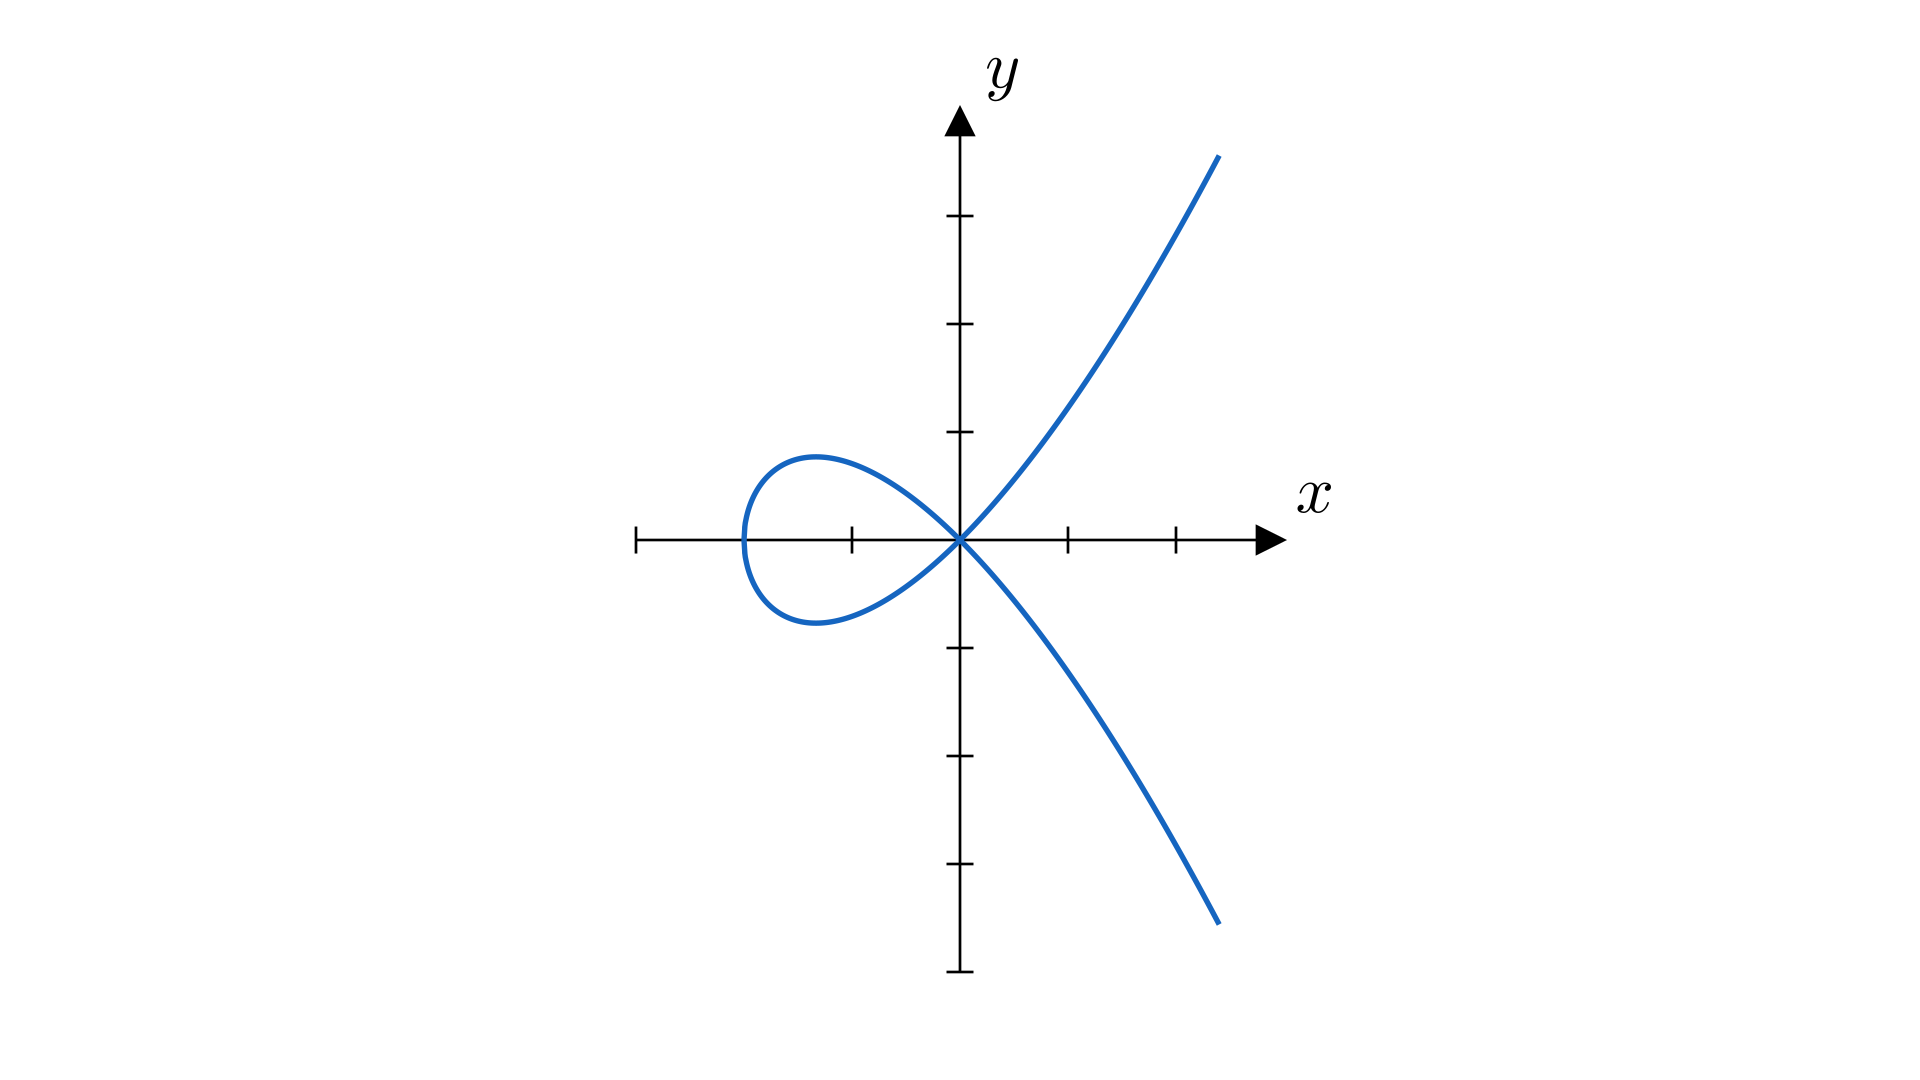
\includegraphics[width=.7\textwidth]{assets/EllipticCurve2D.png}
    % \begin{tikzpicture}[scale=0.85]
    %     \definecolor{curveblue}{RGB}{27,101,187}
    %     \draw[->] (-1.7,0)--(2.4,0) node[right]{\scriptsize$x$};
    %     \draw[->] (0,-2.4)--(0,2.4) node[above]{\scriptsize$y$};
    %     \draw[red!60,dashed] (-1.3,-1.3)--(1.3,1.3) node[above right]{\scriptsize$y=x$};
    %     \draw[red!60,dashed] (-1.3,1.3)--(1.3,-1.3) node[below right]{\scriptsize$y=-x$};
    %     \draw[curveblue,thick,domain=-1.55:1.55,samples=160,smooth,variable=\t]
    %         plot ({\t*\t-1},{\t*\t*\t-\t});
    %     \fill (0,0) circle (1.4pt);
    % \end{tikzpicture}

    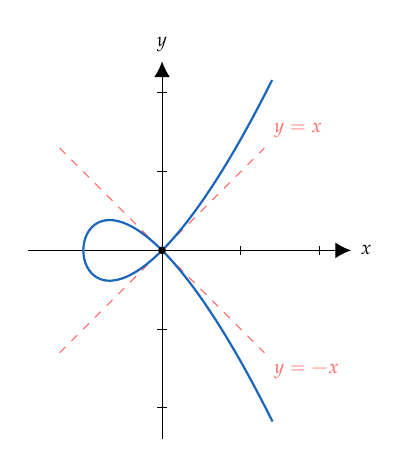
\begin{tikzpicture}[scale=1]
    \usetikzlibrary{arrows.meta}
    \definecolor{curveblue}{RGB}{27,101,187}

    % axes
    \draw[-{Latex[length=2mm,width=2mm]}]
        (-1.7,0)--(2.4,0) node[right]{\scriptsize $x$};

    \draw[-{Latex[length=2mm,width=2mm]}]
        (0,-2.4)--(0,2.4) node[above]{\scriptsize $y$};

    % ticks
    \foreach \x in {-1,1,2}
        \draw (\x,0.06)--(\x,-0.06);

    \foreach \y in {-2,-1,1,2}
        \draw (0.06,\y)--(-0.06,\y);

    % asymptotes
    \draw[red!60,dashed] (-1.3,-1.3)--(1.3,1.3)
        node[above right]{\scriptsize $y=x$};

    \draw[red!60,dashed] (-1.3,1.3)--(1.3,-1.3)
        node[below right]{\scriptsize $y=-x$};
    % curve
    \draw[curveblue,thick,domain=-1.55:1.55,samples=160,smooth,variable=\t]
        plot ({\t*\t-1},{\t*\t*\t-\t});

    \fill (0,0) circle (1.4pt);
\end{tikzpicture}
    \caption{\footnotesize The nodal cubic $y^2 = x^3 + x^2$. The two branches
    cross at the origin with distinct tangent lines $y=x$ and $y=-x$.}
\end{wrapfigure}


We care about studying varieties, and singularities are an obstruction to that. Intuitively, a singularity is a point of the variety where the tangent is not well defined. For instance, in $\A^2$ the curve $y^2 = x^3 + x^2$ has a node at the origin, where two branches cross and there are two perfectly valid tangent directions, $y = x$ and $y = -x$.

Blowups are a systematic tool for resolving singularities like this one. The idea is fairly straightforward: instead of picking one tangent direction at the singular point, we replace the point with a copy of $\P^1$, which parametrizes all lines through it simultaneously. The two branches then lift to the blowup as separate smooth curves, meeting $\P^1$ at different points.

In general, the blowup of a variety $X \subset \A^n$ at a point replaces that point with a copy of $\P^{n-1}$, recording all the directions from which one can approach it. So it lives in $\A^n \times \P^{n-1}$.

Projective space $\P^n$ parametrizes lines through the origin in $\A^{n+1}$: a point $[p_0 : p_1 : \cdots : p_n]$ represents the line through $0$ and $(p_0, \ldots, p_n)$, with two points identified if they differ by a nonzero scalar. A polynomial $f$ therefore defines a well-defined vanishing locus in $\P^n$ only when it is homogeneous, since then $f(\lambda x) = \lambda^d f(x)$ and vanishing is independent of the chosen representative. Subvarieties of $\P^n$ are thus cut out by homogeneous ideals. For the homogeneous coordinate ring $k[x_0, \ldots, x_n]$ of $\P^n$, the dictionary sends a homogeneous radical ideal (other than the irrelevant ideal $(x_0, \ldots, x_n)$, which gives $\varnothing$) to a projective subvariety; for example,
\begin{itemize}[topsep=2pt,itemsep=1pt]
    \item $(0)$ --- all of $\P^n$ (as a set, $\V(0) = \P^n$);
    \item $(x_i)$ --- a hyperplane $\{x_i = 0\} \iso \P^{n-1}$;
    \item $(x_i, x_j)$ --- a codimension-$2$ linear subspace $\{x_i = x_j = 0\} \iso \P^{n-2}$;
    \item $(f)$ for irreducible homogeneous $f$ of degree $d$ --- a hypersurface of dimension $n-1$ (codimension $1$, \emph{regardless of $d$}). This is in general \emph{not} isomorphic to a projective space: a smooth plane cubic ($n=2$, $d=3$) is an elliptic curve, not a $\P^k$.
\end{itemize}

\newpage

\section{Graded Rings and Modules}
Since subvarieties of $\P^n$ are cut out by homogeneous ideals, we need a framework to work with them. The polynomial ring $R = k[x_1, \ldots, x_n]$ decomposes naturally by degree,
\[R = \bigoplus_{d \geq 0} k[x_1, \ldots, x_n]_d,\]
where $R_d = k[x_1, \ldots, x_n]_d$ denotes the homogeneous polynomials of degree $d$. Multiplication respects this decomposition, $R_d \cdot R_e \subseteq R_{d+e}$, and such an $R = \bigoplus_{d \geq 0} R_d$ is called a graded ring. The polynomial ring has a natural grading by degree, but a general ring does not. To extract a graded ring from $R$, we choose ideals $I_i \subseteq R$ forming a descending multiplicative chain,
\[R \supseteq I_1 \supseteq I_2 \supseteq I_3 \supseteq \cdots, \qquad I_i I_j \subseteq I_{i+j}.\]
When the $I_i$ are powers of a single ideal, this chain is called an $I$-adic filtration, and it lets us measure ``how deeply'' an element lies in $I$. For our purposes $I$ is always the maximal ideal of a local Noetherian ring $R$.

From this filtration we recover the associated graded ring $\gr_I R$,
\[\gr_I R := R/I \oplus I/I^2 \oplus I^2/I^3 \oplus \cdots,\]
with a well-defined multiplication: for $a \in I^n/I^{n+1}$ and $b \in I^m/I^{m+1}$ we pick representatives $a' \in I^n$ and $b' \in I^m$ and define $ab \in I^{n+m}/I^{n+m+1}$ to be the image of $a'b'$. One checks this is well defined modulo $I^{m+n+1}$. We now develop some theory around filtrations and graded rings that will be useful later.

The idea of $I$-adic filtrations generalizes to modules.
\begin{definition}
    Given an $R$-module $M$ and an ideal $I \subseteq R$, we get the $I$-adic filtration of the module,
    \[M \supseteq IM \supseteq I^2M \supseteq \cdots,\]
    and the associated graded module,
    \[\gr_I M := M/IM \oplus IM/I^2M \oplus I^2M/I^3M \oplus \cdots,\]
    a graded $\gr_I R$-module: for $a \in I^n/I^{n+1}$ and $b \in I^mM/I^{m+1}M$ we pick representatives $a' \in I^n$, $b' \in I^mM$ and let $ab \in I^{n+m}M/I^{n+m+1}M$ be the image of $a'b'$.
\end{definition}

\begin{remark}
    Intersecting the terms of the $I$-adic filtration of $M$ with a submodule $M' \subseteq M$ generally does \emph{not} give the $I$-adic filtration of $M'$.
\end{remark}

The Artin--Rees lemma characterizes exactly when this does hold. We state it now and prove it once the requisite theory is in place.

\begin{lemma}[Artin--Rees]
    Let $R$ be a Noetherian ring, $I \subseteq R$ an ideal, and $M' \subseteq M$ finitely generated $R$-modules. If
    \[M = M_0 \supseteq M_1 \supseteq M_2 \supseteq \cdots\]
    is an $I$-stable filtration, then the induced filtration
    \[M' = M' \cap M_0 \supseteq M' \cap M_1 \supseteq M' \cap M_2 \supseteq \cdots\]
    is also $I$-stable; that is, there exists $m$ with $I(M' \cap M_n) = M' \cap M_{n+1}$ for all $n \geq m$.
\end{lemma}

\begin{definition}
    Let $R$ be a ring, $I \subseteq R$ an ideal, and $M$ an $R$-module. A filtration $M = M_0 \supseteq M_1 \supseteq \cdots$ is an $I$-filtration if $IM_n \subseteq M_{n+1}$ for all $n \geq 0$, and is $I$-stable if there exists $m$ with $M_{m+i} = I^i M_m$ for all $i \geq 0$.
\end{definition}

\begin{notation}
    We write $M_k$ for $I^kM$, and
    \[\gr_I R = \bigoplus_{k \geq 0} I^k/I^{k+1}, \qquad \gr_I M = \bigoplus_{k \geq 0} M_k/M_{k+1}\]
    for the associated graded ring and module. We also need the \emph{Rees algebra} (studied in detail in \S3) and \emph{Rees module}: for an $I$-filtration $\mathcal{J}: M = M_0 \supseteq M_1 \supseteq \cdots$,
    \[B_I R := \bigoplus_{n \geq 0} I^n t^n \subseteq R[t], \qquad B_{\mathcal{J}} M := \bigoplus_{n \geq 0} M_n\, t^n,\]
    where $B_{\mathcal{J}}M$ is a graded $B_I R$-module. (When $\mathcal{J}$ is the $I$-adic filtration, $M_n = I^n M$.)
\end{notation}

There is no canonical ring homomorphism $R \to \gr_I R$ lifting the structure of $R$. The only canonical ring map out of $R$ compatible with the grading is the projection onto degree $0$,
\[R \twoheadrightarrow R/I = (\gr_I R)_0 \hookrightarrow \gr_I R,\]
which forgets everything in positive degree. The genuinely useful gadget attached to the associated graded is instead a \emph{set} map (not a ring homomorphism), the initial form.

\begin{definition}
    Let $f \in M$ and let $m$ be the greatest integer with $f \in M_m$. The initial form of $f$ is
    \[\init(f) = f \pmod{M_{m+1}} \in M_m/M_{m+1} \subseteq \gr_I M,\]
    or $\init(f) = 0$ if $f \in \bigcap_{m} M_m$.
\end{definition}

\begin{definition}
    For a submodule $M' \subseteq M$, define $\init(M')$ to be the $\gr_I R$-submodule of $\gr_I M$ generated by $\init(f)$ for all $f \in M'$.
\end{definition}

\begin{remark}\label{rem:initials}
    The initial-form map is not additive, and it is not multiplicative when $\gr_I R$ has zero-divisors; in particular $\init(M')$ is generally \emph{not} the submodule generated by the initial forms of a generating set of $M'$.

    For instance, take $R = k[x,y]$, $I = (x,y)$, and $J = (x^2 + y^3, xy) \subseteq R$ with the $I$-adic filtration. The initial forms of the generators are $\init(x^2 + y^3) = x^2$ and $\init(xy) = xy$, so they generate $(x^2, xy) \subseteq \gr_I R \cong k[x,y]$. However,
    \[y \cdot (x^2 + y^3) - x \cdot (xy) = x^2y + y^4 - x^2y = y^4 \in J,\]
    so $\init(y^4) = y^4 \in \init(J)$. But $y^4 \notin (x^2, xy)$, since every element of $(x^2, xy)$ has $x$ as a factor while $y^4$ does not. Hence $\init(J) \supsetneq (\init(x^2 + y^3), \init(xy))$.
\end{remark}

\begin{proposition}\label{prop:stable}
    Let $R$ be a ring, $I \subseteq R$ an ideal, and $M$ a finitely generated $R$-module with an $I$-filtration $\mathcal{J} : M = M_0 \supseteq M_1 \supseteq \cdots$ by finitely generated modules $M_i$. Then $\mathcal{J}$ is $I$-stable if and only if the $B_I R$-module $B_{\mathcal{J}}M$ is finitely generated.
\end{proposition}

\begin{proof}
    ($\Rightarrow$) Assume $\mathcal{J}$ is $I$-stable, so $M_{n+i} = I^i M_n$ for some $n$ and all $i \geq 0$; that is, for $k > n$, $M_k$ is obtained from $M_n$ by multiplying by powers of $I$. Since each of $M_0, \ldots, M_n$ is finitely generated, the union of their generating sets (placed in their respective degrees) gives a finite generating set for $B_{\mathcal{J}}M$.

    ($\Leftarrow$) Assume $B_{\mathcal{J}}M$ is finitely generated. Since $B_{\mathcal{J}}M = \bigoplus_{n \geq 0} M_n\,t^n$ is a direct sum, each generator has only finitely many nonzero homogeneous components, so each generator lies in $M_0 \oplus \cdots \oplus M_{k_i}$ for some $k_i$. Replacing the generators by their homogeneous pieces (which still generate), we may assume $B_{\mathcal{J}}M$ is generated by homogeneous elements lying in degrees $\leq n$, where $n = \max_i k_i$.

    Now take any element of $M_{n+i}$ for $i \geq 0$. As a degree-$(n+i)$ element of $B_{\mathcal{J}}M$, it is a sum of terms $a \cdot m$ with $m$ a generator in some degree $k \leq n$ and $a \in (B_I R)_{n+i-k} = I^{n+i-k}$. Write $a \cdot m = I^i \cdot (I^{n-k} m)$; since $\mathcal{J}$ is an $I$-filtration, $I^{n-k} m \in M_n$, so $a\cdot m \in I^i M_n$. Hence $M_{n+i} \subseteq I^i M_n$. The reverse inclusion is immediate, so $M_{n+i} = I^i M_n$ for all $i \geq 0$ and $\mathcal{J}$ is $I$-stable.
\end{proof}

\begin{proof}[Proof of Artin--Rees]
    Let
    \[\mathcal{J}' : M' = M_0' \supseteq M_1' := M' \cap M_1 \supseteq M_2' := M' \cap M_2 \supseteq \cdots\]
    be the induced filtration on $M'$. Then $B_{\mathcal{J}'}M' = \bigoplus_{n \geq 0} (M' \cap M_n)\,t^n$ is a graded $B_I R$-submodule of $B_{\mathcal{J}}M$.

    Since $\mathcal{J}$ is $I$-stable, $B_{\mathcal{J}}M$ is finitely generated as a $B_I R$-module by Proposition~\ref{prop:stable}. As $R$ is Noetherian and $I$ is finitely generated, $B_I R = \bigoplus_{n \geq 0} I^n t^n$ is a finitely generated $R$-algebra, hence a quotient of a polynomial ring over $R$ and so Noetherian by the Hilbert basis theorem. Therefore the submodule $B_{\mathcal{J}'}M'$ of the finitely generated $B_I R$-module $B_{\mathcal{J}}M$ is itself finitely generated, and Proposition~\ref{prop:stable} (applied to $M'$) shows $\mathcal{J}'$ is $I$-stable.
\end{proof}

\begin{remark}
    A key payoff of the associated graded construction: when $I = \fm$ is the maximal ideal of a Noetherian local ring, $\gr_{\fm} R$ is a finitely generated {graded} algebra over the field $R/\fm$, i.e.\ a quotient of a polynomial ring by a homogeneous ideal. This matters because such algebras are exactly the homogeneous coordinate rings of projective schemes, so passing to $\gr_{\fm} R$ lets us deploy the full toolkit of projective geometry --- $\Proj$, Hilbert functions, Hilbert polynomials, dimension, multiplicity --- on an object built from an otherwise unstructured local ring. Crucially, the passage $R \rightsquigarrow \gr_{\fm} R$ preserves the local numerical invariants we care about: $\dim R = \dim \gr_{\fm} R$, and the Hilbert--Samuel function $n \mapsto \ell(R/\fm^n)$ of $R$ is computed by the Hilbert function of $\gr_{\fm} R$. So dimension and multiplicity can be read off the much more tractable graded ring, and geometrically $\Spec \gr_{\fm} R$ is the tangent cone --- the linearization of $\Spec R$ at the point.
\end{remark}

\newpage

\section{Blowup Algebras}

\begin{definition}
    Let $R$ be a ring and $I \subseteq R$ an ideal. The \textbf{blowup algebra} (Rees algebra) of $I$ in $R$ is the $R$-algebra
    \[B_I R := \bigoplus_{n \geq 0} I^n t^n = R \oplus It \oplus I^2t^2 \oplus \cdots \iso R[It] \subseteq R[t],\]
    where $t$ is a formal variable tracking the power of $I$. The associated graded ring is obtained by quotienting by $IB_IR$:
    \[B_I R / I B_I R = \gr_I R = R/I \oplus I/I^2 \oplus \cdots.\]
\end{definition}

The blowup algebra is the algebraic structure behind the geometric operation of blowing up a subvariety. Suppose $R$ is the coordinate $k$-algebra of an affine variety $X$, and $I \subseteq R$ is the ideal of a subvariety $Y \subseteq X$. Let $a_1, \ldots, a_r$ be $k$-algebra generators for $R$ and $g_0, \ldots, g_s$ generators of $I$ as an ideal of $R$.

\begin{proposition}\label{prop:blowimage}
    The blowup algebra $B_I R$ is a homomorphic image of $k[x_1, \ldots, x_r, y_0, \ldots, y_s]$.
\end{proposition}

\begin{proof}
    Define a ring homomorphism
    \[\phi: k[x_1, \ldots, x_r, y_0, \ldots, y_s] \to B_I R, \quad x_i \mapsto a_i, \quad y_j \mapsto g_j t.\]
    This is surjective: any element of $B_I R$ is a finite sum of terms $f \cdot g\,t^n$ with $f \in R$, $g \in I^n$, and since $f$ is a polynomial in the $a_i$ and $g$ is a polynomial in the $g_j$, every such term is in the image. By the first isomorphism theorem,
    \[B_I R \iso k[x_1, \ldots, x_r, y_0, \ldots, y_s] / \ker(\phi).\]
    Since $B_I R$ is graded (by the power of $t$) and $\phi$ respects the grading, sending the $x_i$ to degree $0$ and the $y_j$ to degree $1$, the kernel is a homogeneous ideal.
\end{proof}

Here $k[x_1,\ldots,x_r]$ is the coordinate ring of $\A^r$ and $k[y_0, \ldots, y_s]$ is the homogeneous coordinate ring of $\P^s$, so $k[x_1, \ldots, x_r, y_0, \ldots, y_s]$ is the coordinate ring of $\A^r \times \A^{s+1}$. Quotienting by a homogeneous ideal in the $y_j$ makes vanishing scale-invariant in the $y_j$ and cuts out a subvariety that is projective in the $y$-directions,
\[Z = \V(\ker \phi) \subseteq \A^r \times \P^s.\]
The projection $\pi: \A^r \times \P^s \to \A^r$ restricts to a map $Z \to X$ which is an isomorphism away from the preimage of $Y$. The set $Z = \Proj(B_I R)$ is the \textbf{blowup of $Y$ in $X$}, and $\pi^{-1}(Y) \subseteq Z$ is the \textbf{exceptional set}.

Algebraically, the exceptional set comes from killing $I$ inside the blowup algebra: $B_I R / I B_I R = \gr_I R$, so
\[\pi^{-1}(Y) = \Proj(\gr_I R) \subseteq \P^s.\]
Recall that $\gr_I R = \bigoplus_{n \geq 0} I^n/I^{n+1}$ is a graded ring, and its homogeneous primes not containing the irrelevant ideal $(\gr_I R)_{>0}$ correspond to points of a projective variety, exactly as for $k[y_0,\ldots,y_s]$ and $\P^s$. This variety --- the projectivized normal cone of $Y$ in $X$ --- parametrizes the limiting directions of approach to $Y$ inside $X$: when $Y$ is the origin in $X \subseteq \A^r$ it is the projectivized tangent cone, with one point for each limiting direction of a secant line to $X$ through $Y$. We make this precise in \S4.

We can now revisit the example from the start of the note more formally.

\subsection*{Example: blowing up the node of $y^2 = x^3 + x^2$}

The curve $X = \V(y^2 - x^3 - x^2)$ has a node at the origin. With $f = y^2 - x^3 - x^2$, the Jacobian $(\partial_x f, \partial_y f) = (-3x^2 - 2x,\; 2y)$ vanishes at $(0,0)$, and $f(0,0)=0$, so the origin is singular.

Blow up $Y = \{0\}$ inside $X$. The coordinate ring is $R = k[x,y]/(y^2 - x^3 - x^2)$, and the maximal ideal of the origin is $I = (x, y)$. Both $R$ (as a $k$-algebra) and $I$ (as an ideal) are generated by $x, y$, so by Proposition~\ref{prop:blowimage} the blowup algebra is the image of $k[x_1, x_2, y_0, y_1]$ under
\[\phi: x_1 \mapsto x, \quad x_2 \mapsto y, \quad y_0 \mapsto xt, \quad y_1 \mapsto yt.\]
Two relations are visibly in $\ker\phi$: the \emph{curve relation} $F = x_2^2 - x_1^3 - x_1^2$, and the \emph{incidence relation} $G = x_1 y_1 - x_2 y_0$, since $\phi(G) = x\cdot yt - y\cdot xt = 0$. Both are homogeneous of degree $\leq 1$ in $y_0, y_1$, so they cut out a subset of $\A^2 \times \P^1$.

\begin{remark}[A subtlety worth flagging]
    $F$ and $G$ do \emph{not} generate $\ker\phi$, and $\V(F,G)$ is \emph{not} the blowup. Setting $x=y=0$ kills both $F$ and $G$, so $\V(F,G)$ contains the entire exceptional line $\{0\}\times\P^1$; in fact $\V(F,G) = \pi^{-1}(X)$ is the reducible \emph{total transform} $\widetilde X \cup (\{0\}\times\P^1)$. The blowup $\Bl_0 X = \Proj(B_I R) = \widetilde X$ is the irreducible \emph{strict transform}: the unique component dominating $X$, obtained by saturating $(F,G)$ with respect to the irrelevant ideal $(y_0, y_1)$ (i.e.\ removing the exceptional component). Concretely, $\ker\phi$ contains further relations; for example
    \[\phi\big(y_1^2 - (1+x_1)y_0^2\big) = (yt)^2 - (1+x)(xt)^2 = (y^2 - x^2 - x^3)t^2 = 0,\]
    and $y_1^2 - (1+x_1)y_0^2$ does \emph{not} vanish on all of $\{0\}\times\P^1$ --- it cuts the exceptional line down to the points that genuinely lie on the blowup.
\end{remark}

It is cleanest to compute the strict transform in the two standard charts of $\Bl_0 \A^2 = \V(xv - yu) \subseteq \A^2 \times \P^1_{[u:v]}$ (here $[u:v]$ are the coordinates with $u \leftrightarrow xt$, $v \leftrightarrow yt$, so $[u:v]=[x:y]$ off the origin):
\begin{itemize}[topsep=2pt,itemsep=2pt]
    \item \emph{Chart $u \neq 0$.} Set $u=1$ and let $m = v$, so $y = mx$. Substituting into $y^2 = x^3+x^2$ gives
    \[m^2x^2 = x^2(x+1) \;\Longrightarrow\; x^2(m^2 - x - 1) = 0.\]
    The factor $x^2$ is the exceptional divisor; the strict transform is $m^2 = x+1$, i.e.\ $x = m^2-1,\ y = m^3 - m$ --- a smooth curve parametrized by $m$. It meets the exceptional divisor $x=0$ at $m = \pm 1$.
    \item \emph{Chart $v \neq 0$.} Symmetrically, with $n = u/v$ and $x = ny$ one gets $y^2(1 - n^2 - n^3 y)=0$; the strict transform meets the exceptional divisor at the same two points (and avoids the vertical direction $[0:1]$).
\end{itemize}
So blowing up separates the branches: the strict transform is smooth and meets the exceptional $\P^1$ in the two points $[u:v] = [1:1]$ and $[1:-1]$, i.e.\ the directions $y = x$ and $y = -x$. These two points are exactly the exceptional set $\pi^{-1}(0)\cap \widetilde X$, which we identify with $\Proj(\gr_I R)$ in \S4.

\newpage


Algebraically, the exceptional set is what remains after setting the affine coordinates to zero: it is the projective variety in $\P^s$ cut out by the relations of $\ker\phi$ with $x_1 = \cdots = x_r = 0$. Equivalently, killing $I$ in the blowup algebra leaves $B_I R / I B_I R = \gr_I R$, and the exceptional set is the projective variety defined by these (homogeneous) relations. This variety (the projectivized normal cone of $Y$ in $X$) parametrizes the limiting directions of approach to $Y$ inside $X$: when $Y$ is the origin in $X \subseteq \A^r$ it is the projectivized tangent cone, with one point for each limiting direction of a secant line to $X$ through $Y$. We make this precise in Section 4.
 
\subsection*{Charts of the blowup}
 
We realized the blowup concretely as the subvariety $Z = \V(\ker\phi) \subseteq \A^r \times \P^s$. To compute with it we cover it by affine pieces, exactly as one covers $\P^s$ by the standard charts $\{y_j \neq 0\}$. We spell this out for a point in affine space, the case we need.
 
Take $X = \A^n$ with coordinates $x_1, \ldots, x_n$ and $Y = \{0\}$, so $I = (x_1, \ldots, x_n)$. The blowup sits in $\A^n \times \P^{n-1}$, with $\P^{n-1}$ carrying coordinates $[u_1 : \cdots : u_n]$ (here $u_i \leftrightarrow x_i t$). The relations $x_i u_j = x_j u_i$ say that the point $(x_1, \ldots, x_n)$ and the direction $(u_1, \ldots, u_n)$ are proportional, so the blowup of $\A^n$ at the origin, denoted as $\Bl_0 \A^n$, is the incidence variety of points and the lines through them,
\[\Bl_0 \A^n = \big\{(p, [\ell]) \in \A^n \times \P^{n-1} : p \in \ell\big\} = \V\big(x_i u_j - x_j u_i : i < j\big) \subseteq \A^n \times \P^{n-1}.\]
(For $X = \A^n$ these incidence relations already generate $\ker\phi$: since $\A^n$ is smooth there is no exceptional component to discard, in contrast to the node below.)
 
\begin{definition}[Affine charts]\label{def:charts}
On the standard chart $U_i = \{u_i \neq 0\}$ of $\P^{n-1}$, dehomogenize by setting $u_i = 1$ and writing $m_j = u_j / u_i$ for $j \neq i$. The relations $x_j u_i = x_i u_j$ become $x_j = m_j x_i$, so every coordinate is a polynomial in $x_i$ and the $m_j$. Hence the $i$-th chart of $\Bl_0 \A^n$ is itself an affine space,
\[\Bl_0 \A^n \cap (\A^n \times U_i) \;\iso\; \A^n \text{ with coordinates } (x_i,\ m_j)_{j \neq i},\]
and in these coordinates the projection $\pi$ is
\[\pi(x_i, (m_j)_{j \neq i}) = (x_1, \ldots, x_n), \qquad x_j = m_j x_i \ (j \neq i).\]
In this chart the exceptional divisor $E = \pi^{-1}(0)$ is the coordinate hyperplane $\{x_i = 0\}$, and the $n$ charts glue along $E$ to recover $E \iso \P^{n-1}$.
\end{definition}
 
For $n = 2$, writing $[u:v]$ for $\P^1$, there are two charts:
\[
\{u \neq 0\}:\ \ m = \tfrac{v}{u},\ \ y = mx,\ \ \text{coords } (x,m),\ \ \pi(x,m) = (x,\,mx),\ \ E = \{x = 0\};
\]
\[
\{v \neq 0\}:\ \ n = \tfrac{u}{v},\ \ x = ny,\ \ \text{coords } (y,n),\ \ \pi(y,n) = (ny,\,y),\ \ E = \{y = 0\}.
\]
 
To blow up a plane curve $X = \V(f) \subseteq \A^2$ through the origin, we pull $f$ back to each chart. Write $f = f_{m_0} + f_{m_0 + 1} + \cdots$ in homogeneous parts with $f_{m_0} = \init(f) \neq 0$, so $m_0 = \ord_0(f)$ is the multiplicity of $X$ at $0$. In the chart $\{u \neq 0\}$, since $f_d(x, mx) = x^d f_d(1,m)$,
\[f(x, mx) = \sum_{d \geq m_0} x^d f_d(1,m) = x^{m_0}\Big(\underbrace{\init(f)(1,m)}_{= \, f_{m_0}(1,m)} + x\,(\cdots)\Big).\]
The factor $x^{m_0}$ is the exceptional divisor taken with multiplicity $m_0$ --- the part of the pullback supported over $0$, giving the \emph{total transform} $\pi^{-1}(X)$ --- and the remaining factor $\widetilde f(x,m)$ cuts out the \emph{strict transform}, the closure $\widetilde X = \overline{\pi^{-1}(X \setminus 0)}$. Setting $x = 0$, the strict transform meets the exceptional divisor exactly where
\[\init(f)(1,m) = 0,\]
i.e.\ at the projectivized zeros of the initial form: the tangent directions of $X$ at $0$. This is the geometric shadow of the tangent cone theorem of \S4.
 
 
\subsection*{Blowing up the node of $y^2 = x^3 + x^2$}
 
\begin{wrapfigure}{r}{0.5\textwidth}
    \centering
    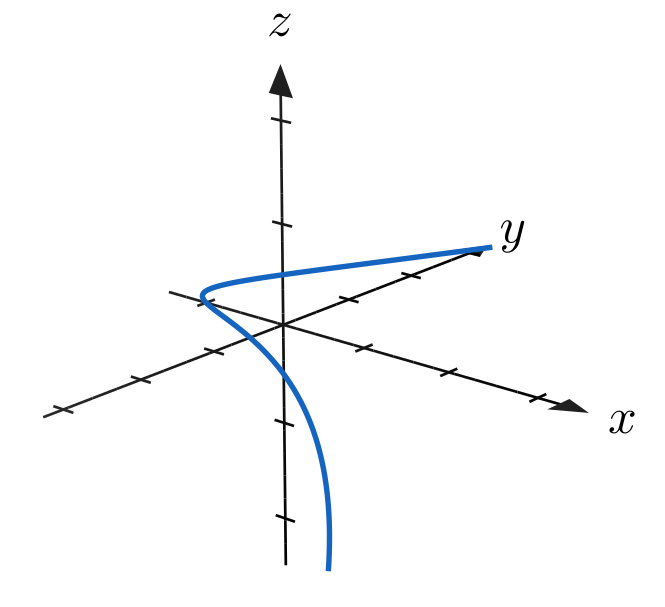
\includegraphics[width=.5\textwidth]{assets/EllipticCurve3D_ManimCE_v0.20.1.png}
    \caption{\footnotesize The strict transform of the node in the slope chart $\A^2_{x,y} \times \A^1_z$ of the blowup, where the vertical coordinate is the slope $z = y/x$. The smooth space curve $z \mapsto (z^2 - 1,\ z^3 - z,\ z)$ has no self-intersection; projecting it to the $xy$-plane (forgetting $z$) collapses it onto the nodal cubic, regluing the points $z = +1$ and $z = -1$ at the origin. Blowing up has lifted the two branches to the heights $z = \pm 1$, the tangent slopes $y = \pm x$.}
    \label{fig:strict-transform}
\end{wrapfigure}
 
The curve $X = \V(f)$ with $f = y^2 - x^3 - x^2$ has a node at the origin: the Jacobian $(\partial_x f, \partial_y f) = (-3x^2 - 2x,\ 2y)$ vanishes at $(0,0)$ and $f(0,0) = 0$, and the lowest-degree part $\init(f) = y^2 - x^2 = (y-x)(y+x)$ has two distinct linear factors --- multiplicity $m_0 = 2$, with tangent directions $y = \pm x$.
 
We blow up $Y = \{0\}$. The coordinate ring is $R = k[x,y]/\langle y^2 - x^3 - x^2 \rangle$ and the ideal of the origin is $I = \langle x, y \rangle$ (by the Nullstellensatz). Both $R$ and $I$ are generated by $x, y$, so by Proposition~\ref{blowimage} the blowup algebra is the image of $k[x_1, x_2, y_0, y_1]$ under
\[\phi : \begin{cases} x_1 \mapsto x, \\ x_2 \mapsto y, \\ y_0 \mapsto xt, \\ y_1 \mapsto yt. \end{cases}\]
Two relations sit visibly in $\ker\phi$: the curve relation $F = x_2^2 - x_1^3 - x_1^2$ and the incidence relation $G = x_1 y_1 - x_2 y_0$ (since $\phi(G) = x \cdot yt - y \cdot xt = 0$). These cut out a set $Z \subseteq \A^2 \times \P^1$ --- but $F$ and $G$ both vanish at $x = y = 0$, so $\V(F,G)$ contains the entire exceptional line $\{0\} \times \P^1$ and is the reducible total transform.
 
Eliminating $t$ as in Remark~\ref{rem:strict} gives the full kernel,
\[\ker\phi = \big(F,\ G,\ H,\ P\big), \qquad H = x_2 y_1 - (x_1^2 + x_1)y_0, \quad P = y_1^2 - (1 + x_1)y_0^2,\]
(both $H$ and $P$ check out: $\phi(H) = (y^2 - x^3 - x^2)t = 0$ and $\phi(P) = (y^2 - x^2 - x^3)t^2 = 0$). The two extra generators are what trim the exceptional line off the total transform: restricted to $\{0\}\times\P^1$, the relation $P$ becomes $y_1^2 - y_0^2$, which vanishes only at $[y_0 : y_1] = [1:1]$ and $[1:-1]$. The same two points fall out --- more transparently --- from the charts of Definition~\ref{def:charts}.
 
\medskip
\noindent\textit{Chart $\{u \neq 0\}$} (slope $m = v/u$, so $y = mx$). Substituting,
\[f(x, mx) = (mx)^2 - x^3 - x^2 = x^2\big(m^2 - x - 1\big).\]
The factor $x^2$ is the exceptional divisor (multiplicity $m_0 = 2$); discarding it, the strict transform is the closure of the locus with $x \neq 0$, namely
\[\widetilde X : \quad m^2 - x - 1 = 0, \qquad\text{i.e.}\qquad x = m^2 - 1, \quad y = mx = m^3 - m,\]
a \emph{smooth} curve. It meets the exceptional divisor $x = 0$ where $m^2 - 1 = 0$, i.e.\ at $m = \pm 1$ --- the directions $[u:v] = [1:1]$ and $[1:-1]$, exactly the roots of $\init(f)(1,m) = m^2 - 1$.
 
\medskip
\noindent\textit{Chart $\{v \neq 0\}$} ($n = u/v$, so $x = ny$). Substituting,
\[f(ny, y) = y^2 - n^3 y^3 - n^2 y^2 = y^2\big(1 - n^2 - n^3 y\big),\]
with strict transform $1 - n^2 - n^3 y = 0$. It meets $y = 0$ where $1 - n^2 = 0$, i.e.\ at $n = \pm 1$ --- the same two points $[1 : \pm 1]$ --- and misses the vertical direction $[0:1]$ (there $1 = 0$ has no solution).
 
\medskip
So blowing up separates the branches: the strict transform $\widetilde X$ is smooth, and it meets the exceptional $\P^1$ in the two points $[1:1]$ and $[1:-1]$, i.e.\ the tangent directions $y = \pm x$. These two points are the exceptional set $\pi^{-1}(0) \cap \widetilde X$, which we identify with the projectivized tangent cone in \S4.

\section{Tangent Cone}

\begin{theorem}[Krull's Intersection Theorem]
    Let $R$ be a Noetherian ring, $I \subseteq R$ an ideal, and $M$ a finitely generated $R$-module. There exists $r \in I$ with
    \[(1-r) \bigcap_{k=1}^\infty I^kM = 0.\]
\end{theorem}

\begin{proof}
    Let $N = \bigcap_{k=1}^\infty I^k M$; we find $r \in I$ with $(1-r)N = 0$. By Artin--Rees applied to $N \subseteq M$ (with the $I$-adic filtration on $M$), there exists $m$ such that for all $n \geq m$,
    \[N \cap I^n M = I^{n-m}(N \cap I^m M).\]
    In particular $N \cap I^{m+1}M = I(N \cap I^m M)$. But $N \subseteq I^{m+1}M$ and $N \subseteq I^m M$, so $N \cap I^{m+1}M = N$ and $N \cap I^m M = N$, giving $N = IN$. Since $R$ is Noetherian and $M$ is finitely generated, $N$ is finitely generated, and Nakayama's lemma applied to $N = IN$ yields $r \in I$ with $(1-r)N = 0$.
\end{proof}

\begin{corollary}
    Let $R$ be Noetherian. If $R$ is a domain, or $(R, \fm)$ is local, and $I \subsetneq R$, then $\bigcap_{k=1}^\infty I^k = 0$.
\end{corollary}

\begin{proof}
    Take $M = R$, so there is $r \in I$ with $(1-r)\bigcap_k I^k = 0$. As $I$ is proper, $1 \notin I$, so $r \neq 1$ and $1 - r \neq 0$. If $R$ is a domain this forces $\bigcap_k I^k = 0$. If $R$ is local, $r \in I \subseteq \fm$, so $1 - r \notin \fm$ is a unit, again forcing $\bigcap_k I^k = 0$.
\end{proof}

\begin{corollary}
    Let $R$ be a Noetherian local ring and $I \subsetneq R$ an ideal. If $\gr_I R$ is a domain, then so is $R$.
\end{corollary}

\begin{proof}
    Suppose $fg = 0$ in $R$ with $f, g \neq 0$. The product $\init(f)\init(g)$ is, by definition, the image of $fg$ in the relevant graded piece, hence $\init(f)\init(g) = 0$ in $\gr_I R$. As $\gr_I R$ is a domain, $\init(f) = 0$ or $\init(g) = 0$; say $\init(f) = 0$. Then $f \in \bigcap_{k} I^k = 0$ by the previous corollary, so $f = 0$, a contradiction. Hence $R$ is a domain.
\end{proof}

We now make the link between the exceptional set and the associated graded ring geometric. Throughout, $R = k[x_1, \ldots, x_r]/J$ with $I = (x_1, \ldots, x_r)$, $k$ algebraically closed, and $J \subseteq I$ (so the origin lies on $X$); let $X = \V(J) \subseteq \A^r$.

\begin{definition}
    A point $p = (p_1,\ldots,p_r) \in \A^r \setminus \{0\}$ spans a secant line $\overline{0p}$, i.e.\ a direction $[p_1 : \cdots : p_r] \in \P^{r-1}$. The set of \emph{limiting} secant directions,
    \[\P TC_0(X) := \overline{\{[p] : p \in X \setminus \{0\}\}} \subseteq \P^{r-1},\]
    is the \textbf{projectivized tangent cone}. Over $\C$ the closure is genuinely a set of limits: if $p_n \in X\setminus\{0\}$ with $p_n \to 0$, the directions $[p_n]$ have a convergent subsequence because $\P^{r-1}$ is compact. The \textbf{(affine) tangent cone} $TC_0(X) \subseteq \A^r$ is the cone over $\P TC_0(X)$ --- the union of all these lines through the origin (together with $0$). It is the affine version, and the object the theorem below describes; its projectivization $\P TC_0(X)$ is precisely the exceptional set of $\Bl_0 X$ from \S3.
\end{definition}

One shows that the affine tangent cone is cut out by the initial ideal $\init_I(J)$ and that its coordinate ring is $\gr_I R$; this is the content of the next theorem. (For the general theory of tangent cones, associated graded rings, and the Artin--Rees lemma, see Eisenbud, \emph{Commutative Algebra with a View Toward Algebraic Geometry}, Ch.~5, and Harris, \emph{Algebraic Geometry: A First Course}.)

\begin{theorem}\label{thm:tc}
    Let $R = k[x_1, \ldots, x_r]/J$ with $I = (x_1, \ldots, x_r)$, $k$ algebraically closed, and $J \subseteq I$. The (affine) tangent cone to $X = \V(J) \subseteq \A^r$ at the origin is the algebraic set
    \[TC_0(X) = \V(\init_I(J)) \subseteq \A^r,\]
    where $\init_I(J) = \langle \init(f) : f \in J \rangle \subseteq k[x_1, \ldots, x_r]$ is the ideal generated by the initial forms of \emph{all} elements of $J$. Moreover, the coordinate ring of the tangent cone is
    \[k[x_1, \ldots, x_r]/\init_I(J) \iso \gr_I R.\]
\end{theorem}

\begin{proof}
    Let $S = k[x_1, \ldots, x_r]$ and $\fm = (x_1,\ldots,x_r) \subseteq S$, so $R = S/J$ and $I = \fm/J = \fm R$. Each $\init(f)$ is homogeneous, so $\init_I(J)$ is homogeneous and $\V(\init_I(J))$ is a cone. We grade $S$ by degree and define the $k$-algebra map
    \[\phi : S \to \gr_I R, \qquad x_i \mapsto \overline{x_i} \in I/I^2.\]
    Since $S$ is free on the $x_i$ this is well defined, and it is graded because the generators land in degree $1$. It is surjective: $(\gr_I R)_0 = R/I = k$, and as $I$ is generated by the $x_i$, the piece $I^n/I^{n+1}$ is spanned by degree-$n$ monomials in the $\overline{x_i}$, i.e.\ by $\phi(S_n)$.


    We claim $\ker\phi = \init_I(J)$, degree by degree. Under $S_n \iso \fm^n/\fm^{n+1}$, the degree-$n$ part of $\phi$ is the natural surjection
    \[\fm^n/\fm^{n+1} \twoheadrightarrow I^n/I^{n+1} = (\fm^n + J)/(\fm^{n+1}+J) \iso \fm^n/\big(\fm^{n+1} + (J\cap \fm^n)\big),\]
    whose kernel is $\big((J\cap\fm^n) + \fm^{n+1}\big)/\fm^{n+1}$. A degree-$n$ form $g$ lies in this kernel iff $g \equiv h \pmod{\fm^{n+1}}$ for some $h \in J \cap \fm^n$; writing $h = h_n + (\text{higher order})$, this says $g = h_n$, which is $\init(h)$ when $\ord(h)=n$ (and $0$ otherwise). Conversely each such $\init(h)$ is in the kernel. Finally, because $\gr_{\fm} S \iso S$ is a domain, orders add ($\init(g)\init(h) = \init(gh)$), so the degree-$n$ part of the \emph{ideal} $\init_I(J)$ is exactly $\operatorname{span}_k\{\init(h) : h \in J,\ \ord h = n\}$. Hence $\ker\Phi = \init_I(J)$ and
    \[\gr_I R \iso S/\init_I(J).\]
    For $f \in J$ write $f = \init(f) + (\text{higher order})$ with $\ord f = d$. If $[v]$ is a limit of secant directions, say $p_n = t_n v_n \to 0$ with $t_n \to 0$ and $v_n \to v$, then
    \[0 = f(t_n v_n) = t_n^{d}\big(\init(f)(v_n) + t_n(\cdots)\big);\]
    dividing by $t_n^d$ and letting $n \to \infty$ gives $\init(f)(v) = 0$. As this holds for all $f \in J$, every limiting direction lies in $\V(\init_I(J))$, so $TC_0(X) \subseteq \V(\init_I(J))$.

    For the reverse inclusion it is cleanest to use the blowup: by the isomorphism above, the projectivized cone $\P\,\V(\init_I(J)) = \Proj(S/\init_I(J)) = \Proj(\gr_I R)$ is exactly the exceptional fibre $\pi^{-1}(0)$ of $\Bl_0 X \to X$ (\S3). Properness of $\pi$ identifies the points of this fibre with the limiting secant directions, giving $\V(\init_I(J)) \subseteq TC_0(X)$. Over the algebraically closed field $k$ the two cones therefore agree as sets.
\end{proof}

\subsection*{Intuition, and what the proof really needs}

Two ideas drive the theorem, one algebraic and one geometric, and it helps to keep them apart.

The \emph{algebraic engine} is the identity $\gr_I R \iso S/\init_I(J)$. The polynomial ring $S$ \emph{is} its own associated graded $\gr_{\fm} S$, so $\Phi$ is just the map induced on associated graded rings by the quotient $S \twoheadrightarrow R$; passing to $\gr$ replaces each $f \in J$ by its lowest-degree part $\init(f)$. The only real subtlety --- and it is the whole content --- is that the kernel is generated by the initial forms of \emph{all} elements of $J$, not merely of a chosen generating set (recall Remark~\ref{rem:initials}: $\init_I(J)$ can be strictly larger than $(\init f_1, \ldots, \init f_s)$). Computing the kernel degree by degree, as above, is the actual work; the rest is bookkeeping.

The \emph{geometric picture} is that $\init(f)$ is the lowest-order term of $f$ at $0$, so $\V(\init(f))$ is the best homogeneous approximation to $\{f=0\}$ at the origin --- its tangent cone. Intersecting over all $f \in J$ gives the tangent cone of $X$.

Two honest caveats about the proof:
\begin{itemize}[topsep=2pt,itemsep=3pt]
    \item \textbf{The two inclusions are not symmetric.} That a limiting secant direction kills every $\init(f)$ is the easy Taylor expansion above. The converse --- that \emph{every} point of $\V(\init_I(J))$ is realized as a limit of secant lines --- is the substantive direction, and it is \emph{not} ``the same argument backwards.'' It follows from the blowup being proper (its exceptional fibre is $\Proj \gr_I R$), or, over $\C$, from a curve-selection/limit argument. The sequential ``$p_n \to 0$'' language also presupposes a topology: over $\C$ it is literal, but over a general algebraically closed field one replaces limits by the Zariski topology and the valuative criterion --- or simply \emph{defines} $TC_0(X)$ algebraically as $\Spec \gr_I R$.
    \item \textbf{Set versus scheme.} $\init_I(J)$ need not be radical, so the equality $TC_0(X) = \V(\init_I(J))$ is an equality of \emph{sets} (it pins down $\sqrt{\init_I(J)}$). The ``moreover'' --- coordinate ring $= \gr_I R = S/\init_I(J)$ --- is the finer scheme-theoretic statement, and it is the one carrying the multiplicity. For the node below, $\init_I(J) = (y^2 - x^2)$ is radical, so the distinction is invisible there; in general (e.g.\ a cusp) it is not.
\end{itemize}

\begin{example}
    For the nodal cubic $X = \V(y^2 - x^3 - x^2)$, with $f = y^2 - x^3 - x^2$, the lowest-degree part is $\init(f) = y^2 - x^2 = (y-x)(y+x)$. Since $J = (f)$ is principal and orders add in $S$, $\init_I(J) = (\init f) = (y^2 - x^2)$. Hence
    \[TC_0(X) = \V(y^2 - x^2) \subseteq \A^2,\]
    the union of the lines $y = x$ and $y = -x$: the two tangent directions at the node. Its coordinate ring is $k[x,y]/(y^2-x^2) \iso \gr_I R$, and $\Proj$ of it is the two points $[1:1], [1:-1] \in \P^1$, matching the exceptional set of \S3. (The Hilbert function $1, 2, 2, 2, \ldots$ of $\gr_I R$ records multiplicity $2$ --- the node is a double point.)
\end{example}

\end{document}